\section{End of Turn}
\par
After all cards have been played (i.e. the Card Phase is completed for the the year), players must now deal with returning units to their home areas, supply and replacements. This reflects the end of the campaign year when armies returned home or went into winter quarters in effect “wintering”. The End of Turn sequence below should be followed strictly.

\subsection{Check Harvest}
\blockquote[Book V, Chapter 24]{The grain harvest that year in Gaul had been poor because of drought, so I was compelled to change my usual methods of arranging winter quarters for my legions, and distribute them among a larger number of tribes.}
\par
The harvest affects garrison limits for each area at the end of the year. The "garrison limit" is the maximum number of Roman legions that may be stationed in an area. Check the harvest by rolling a die.

On a roll of 1, it’s a poor harvest and the garrison limit for each area is 1 legion. Immediately reduce Roman supply by 2 points.

On a roll of 6, it’s a bountiful harvest and the garrison limit for each area is 3 legions. Immediately increase Roman supply by 2 points.

On a roll of 2-5 the garrison limit for each area is 2, and there is no adjustment to the Roman supply track.

Caesar and Gallic tribe units (including minor leaders) in their home area do not count against the area garrison limit.

\raggedbottom

\subsection{German and Gallic Replacements}
\par
German units in Germania and Gallic tribe units controlled by either player in their home area may add one point strength per unit. Gallic and German units outside of their home area may not receive replacements.

\textit{Note: Since eliminated German and Gallic units are not on the board yet, they do not have the opportunity to receive replacements this turn.}

\begin{samepage}
\subsection{Units Go Home}
\par
Units return to their home areas in the following order:
\begin{enumerate}
  \setlength\itemsep{0em}
  \item {\small Eliminated Gallic units}
  \item {\small Roman legions}
  \item {\small Gallic units controlled by the Roman player}
  \item {\small Gallic units controlled by the Barbarian player}
  \item {\small German units}
\end{enumerate}
\end{samepage}

\subsubsection{Eliminated Gallic Units Return Home}
\label{eliminated_gallic_units_return_home}
\par
Gallic tribe units that were eliminated return to their home area. If the area is occupied by any units, the tribe is now controlled by the owner of the occupying units at strength 1. If the area is not occupied by any units, it returns to neutral status at full strength and the units are placed face down.

\textbf{Exception:} If the Helvetii are eliminated, they are permanently removed from the game. Replace them with the Nantuates unit which returns at full strength (during the "Eliminated Gallic Units Return Home" step), and under the control of any player that occupies the Helvetii area, or face down if neither player does.

\subsubsection{Roman Legions Return Home}
\blockquote[Book V, Chapter 53]{Caesar sent Fabius back to his winter quarters with his own legion, while he himself decided to spend the winter with three legions, each in its own camp, around Samarobriva. Since such formidable Gallic uprisings had occurred, he thought it best to remain personally near the army for the entire winter.}
\par
All Roman legions returning home must return to Transalpine Gaul. If there are enemy units in Transalpine Gaul, then a battle is resolved immediately. All returning legions are considered a single group, and are considered the attackers. Barbarian units eliminated in battle return home as per \ref{eliminated_gallic_units_return_home} and \ref{german_units_return_home}, respectively, at the end of the battle. Roman units may only retreat or regroup to the Off-Map area, if necessary.

Caesar must return home if he stayed outside of Transalpine Gaul at the end of the previous turn. Use the ‘Caesar Wintered’ block on the turn track to remind yourself if and when the Caesar unit remains outside Transalpine Gaul at the end of a year. If Caesar must return to Transalpine Gaul but is stopped because he is unable (or unwilling) to defeat Barbarian units already there, then upon retreat he returns to the off-map area instead.

The Roman player may leave a number of legions in Gallic areas outside of Transalpine Gaul up to the garrison limit of each area. Each legion that does not go home costs Supply points as per \ref{supply_and_attrition}. Each legion suffers a 1 step reduction on its strength if a Supply point cannot be paid, except for the Caesar unit which may stay in any Gallic tribe area at no Supply cost and does not count against an area's garrison limit. Roman legions that have been eliminated do not return immediately, but instead return as reinforcements the following turn. See the Roman Reinforcements section eliminated Roman legions.

Any legions currently in the Off-Map area may move for free into to the Transalpine Gaul area, potentially participating in a battle there as a reserve force.

Legions may not winter in Germania.

\subsubsection{Gallic Units Controlled by the Roman Player Return Home}
\par
Gallic tribe units controlled by the Roman player return home and remain Roman allies. If their home area is occupied by units controlled by the Barbarian player, they switch allegiance to the Barbarian player immediately at current strength.

\subsubsection{Gallic Units Controlled by the Barbarian Player Return Home}
\par
Gallic tribe units, including minor leaders, controlled by the Barbarian player then return to their home area (unless staying outside of their home area with Vercingetorix) and remain Barbarian allies. If the area is occupied by a Roman unit or Roman allied Gallic unit then the tribe defects at current strength to the Roman player. If the home area of a minor leader is occupied by a Roman legion, then the minor leader is eliminated instead. Vercingetorix may return to his home area but is not obligated to, since he can stay outside of his home area every turn. Gallic tribe units may only remain outside of their home area if they remain with Vercingetorix, up to the garrison limit of the area.

\textit{Note: Unlike Caesar, Vercingetorix counts against the area's garrison limit.}

\textbf{Exception:} If the Helvetii unit was eliminated, replace it with the Nantuates unit at full strength instead. These units have been specially marked as a reminder.

\begin{center}
  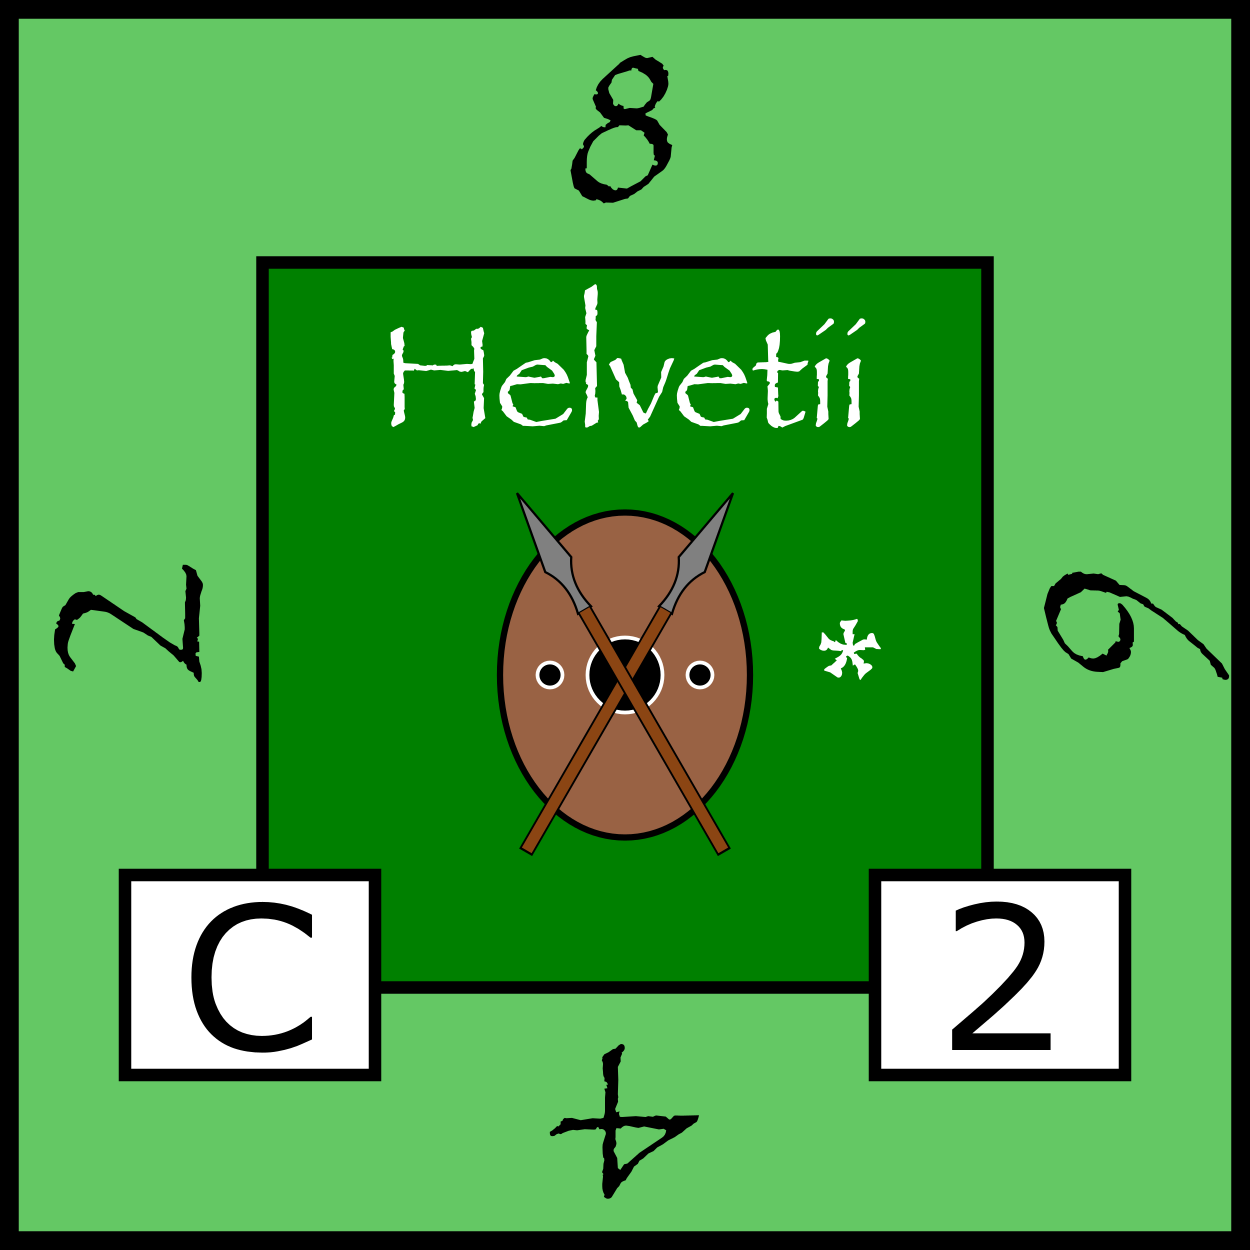
\includegraphics[width=0.40\linewidth]{Helvetii.png}
  \hspace{1mm}
  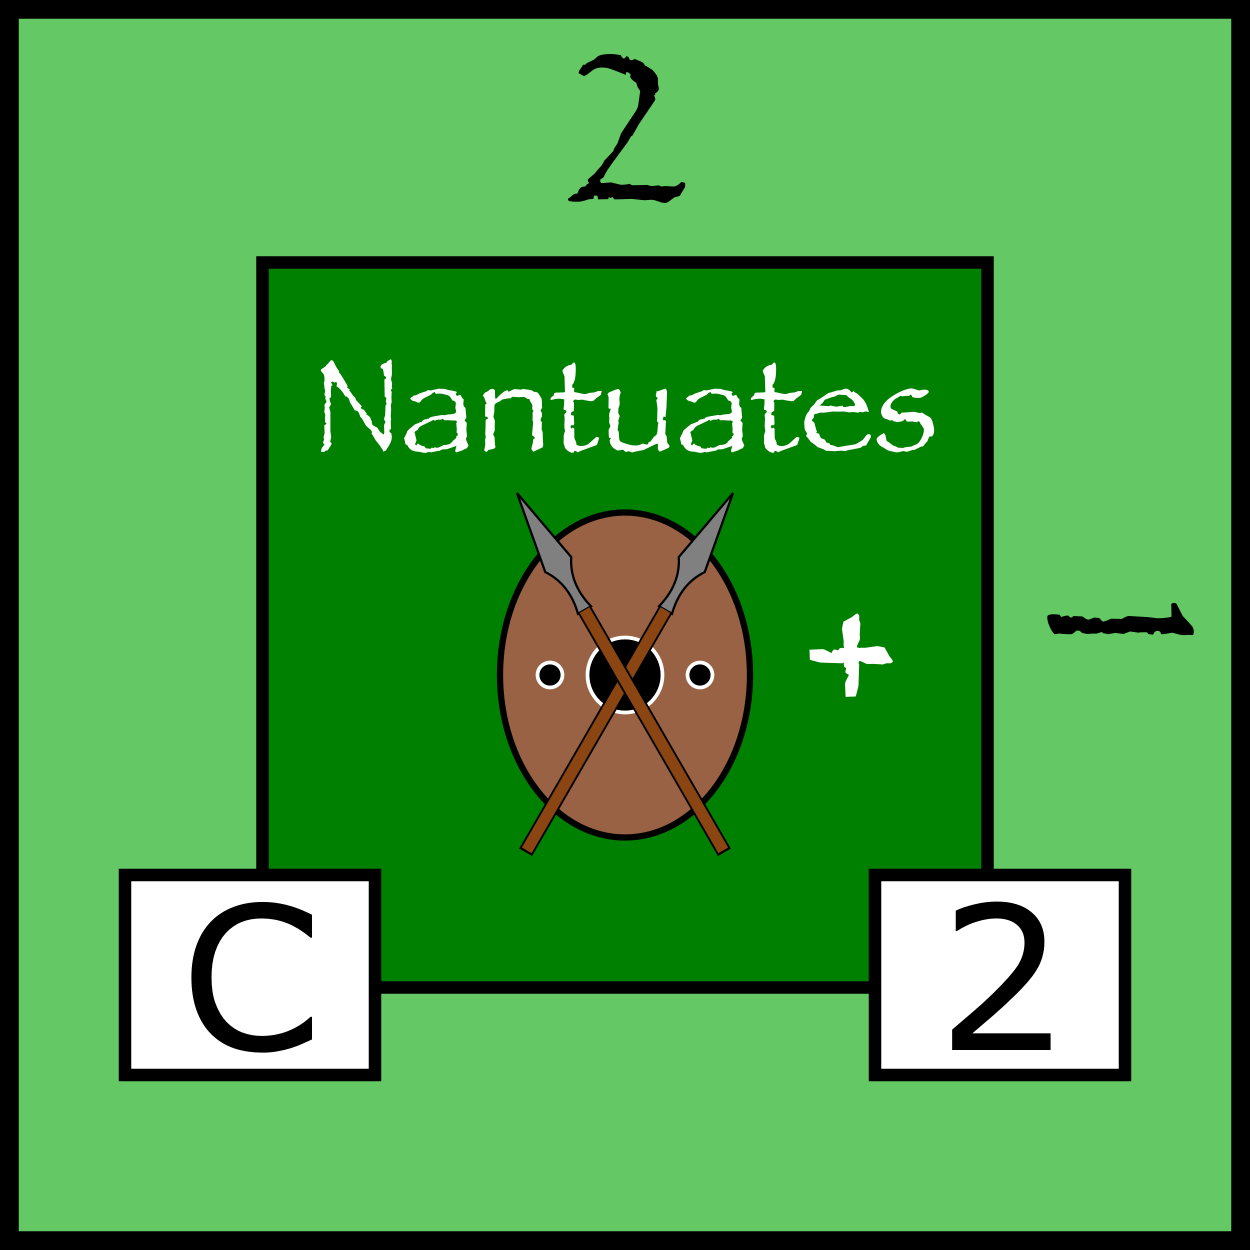
\includegraphics[width=0.40\linewidth]{Nantuates.png}
\end{center}

\subsubsection{German Units Return Home}
\label{german_units_return_home}
\par
German units that were eliminated return to Germania at strength 1. German units (only) may remain with the Ariovistus unit outside of Germania up to the garrison limit of the area. All other German units return home at their current strength.

The Ariovistus unit does count against the area garrison limit. Use the ‘Ariovistus Wintered’ block on the turn track if Ariovistus remains outside of Germania at the end of a year. Ariovistus must return home if he stayed outside of Germania at the end of the previous turn.

\textbf{Note:} Roman and Gallic units, including leaders, may not stay in Germania at the end of a turn.

\subsection{Supply and Attrition}
\label{supply_and_attrition}
\par
The Roman player must now pay Supply points for each Roman legion wintering outside of Transalpine Gaul. It always costs 1 Supply point per legion, regardless of the Harvest level. If enough supply points are not available, each legion that cannot be supplied takes one step reduction through attrition.

The Roman player must attempt to supply all units. Attrition is never voluntary. Any legions reduced to strength 0 from attrition are eliminated and count as victory points for the Barbarian player. Any legion eliminated as the result of attrition will return at the end of the following turn as a reinforcement. See the Roman Reinforcements section at \ref{roman_reinforcements} for more details.

\textit{Note: If this is the last turn, you can skip ahead to Score Victory Points from here.}

\subsection{Roman Replacements}
\par
The Roman player may add strength steps to Roman legions using supply points. Each step added costs one supply point. Legions outside of Transalpine Gaul may only add a maximum of one step per unit. Legions in Transalpine Gaul or the Off-Map area may add strength steps up to their maximum strength.

\subsection{Roman Supply Point Production}
\par
The Roman player now receives one Supply point for each fortified town area he controls, except for Transalpine Gaul and Avaricum, which each produce two Supply points. Adjust the Roman Supply block accordingly. The number of Supply points may never increase above 19, nor decrease below 0.

\subsection{Roman Reinforcements}\label{roman_reinforcements}
\blockquote[Book II, Chapter 2]{This news as well as dispatches prompted Caesar to levy two new legions in Cisalpine Gaul, and by the beginning of the milder season he sent his legate Quintus Pedius to lead them into the interior of Gaul.}
\par
After collecting supply points, the Roman player has up to three new legions that can be constructed. The cost is one supply point per strength point, up to four strength points, maximum (though less if desired). These are legions XIII, XIV, and XV. Normally a maximum of one new legion per turn may be brought in as a reinforcement.

If the Massive Revolt event has been played then two additional units - legions V and VI - may be built by the Roman player, and for the rest of the game up to two legions per turn can be brought in as reinforcements.

Any reinforcements, including eliminated legions returning to play, are placed in the Roman Off-Map area.

\subsubsection{Eliminated Legions}
\par
Any Roman Legions that were eliminated this turn return at the end of the next turn during the Reinforcement Phase at full strength in the Roman Off-Map area. For example, a legion killed on turn 3 (56 BC) would return at the end of turn 4 (55 BC). Players should place eliminated legions on the turn track to indicate when they will return to play.

Legions that are eliminated and return to play in this manner do not require supply points to replace.

\textit{It is assumed that if the legion is destroyed that Caesar received a replacement legion from Rome. This happened historically when 15 cohorts were destroyed in 54 BC, and a legion - borrowed from Pompey - was sent to replace it.}

\subsection{Score Victory Points}
\par
The Roman player now scores victory points for controlled tribes. These points are cumulative with points scored on previous turns.

Each controlled tribal area scores 1 VP for the Roman player. Remember that this does NOT include Transalpine Gaul.

\textit{For VP purposes, this does not include Transalpine Gaul or the Roman off-map area.}

\subsection{Score Optional VP}
If playing with the Yearly Objectives optional rules, score those points as appropriate now. See the section on Yearly Objectives for more details.
